%% Mathematical Programming Computation (Springer) submission version.
%% Generated by scripts/research/build_mpc.py from paper/main.tex: the body is identical and
%% only the editorial frame differs. See paper/mpc/MPC_NOTES.md for the list of changes.
\RequirePackage{fix-cm}
%% envcountsect and envcountsame reproduce the numbering of the original manuscript:
%% one shared counter, numbered within the section (Proposition 4.1, 4.2, ..., Corollary 5.2).
\documentclass[smallextended,envcountsect,envcountsame]{svjour3}
\smartqed
\journalname{Mathematical Programming Computation}
\usepackage[T1]{fontenc}
\usepackage{microtype}
\usepackage{amsmath,amssymb,mathtools}
\usepackage{graphicx,booktabs,tabularx,array,enumitem}
\usepackage[numbers,sort&compress]{natbib}
\usepackage{xurl}
\usepackage[hidelinks]{hyperref}
\usepackage[capitalise,nameinlink,noabbrev]{cleveref}
%% The class defines the theorem-like environments itself, and with envcountsame they all share
%% the "theorem" counter, which is what cleveref keys on. Every theorem-like environment in this
%% paper is a proposition except one corollary, which is never cross-referenced, so naming that
%% counter "Proposition" reproduces the wording of the original manuscript exactly. If a theorem
%% or a reference to the corollary is ever added, this has to be revisited.
\crefname{theorem}{Proposition}{Propositions}
\Crefname{theorem}{Proposition}{Propositions}
\newcommand{\doi}[1]{\href{https://doi.org/#1}{\nolinkurl{https://doi.org/#1}}}
\newcommand{\R}{\mathbb R}
\newcommand{\diag}{\operatorname{diag}}
\newcommand{\norm}[1]{\left\lVert#1\right\rVert}
\newcommand{\abs}[1]{\left|#1\right|}
\newcommand{\argmin}{\operatorname*{arg\,min}}
\newcommand{\nnz}{\operatorname{nnz}}
\graphicspath{{figs/}}
%% The Springer measure is narrower than the original layout; a little stretch absorbs the
%% lines that no longer break as well. No text is changed.
\emergencystretch=1.5em
\begin{document}

\title{Pre-Export Row Scaling for Generated Mixed-Integer Programs: Mechanism Attribution and
Residual-Budget Contracts}
\titlerunning{Pre-Export Row Scaling for Generated MIPs}
\author{Mathias Rodr\'iguez Castro}
\authorrunning{M. Rodr\'iguez Castro}
\institute{M. Rodr\'iguez Castro \at
              Facultad de Ingenier\'ia, Universidad de la Rep\'ublica,
              Montevideo, Uruguay \\
              \email{mathiasr@fing.edu.uy}}
\date{Received: date / Accepted: date}
\maketitle

\begin{abstract}
Multiplying a row of a mixed-integer program by a positive number preserves it exactly and
changes the numbers a solver sees. We ask what that change buys and what it still guarantees.
On 306 generated hydrothermal-dispatch models, holding each model's LP basis fixed across its
representations, geometric-mean row scaling lowers the condition number of the exported file on
every model, by six to eight orders of magnitude in the median of each class. That figure
describes the file: rescaling the same bases with a solver-style row-and-column equilibration
recovers most of it, leaving a factor of a few, and on one class it inverts the ordering of
kernels, so a diagnostic read on
the exported matrix does not rank scaling policies. We then separate two kinds of
information. An apparent block-metadata effect is a coupling-kernel effect, because
geometric-mean centering makes the extrema-based block statistic identically one; a residual
budget in application units, by contrast, survives consistent re-emission, and we characterize
exactly the row factors a budget and coefficient limits admit. In reconstructed dispatch runs, scaling used
30--32\% less solver work on the instances every policy completed, while one timed out under
every scaled policy and reversed the failure-sensitive ordering. In an enumerated stress test,
plain centering lost verified optima on all three solvers and adding the budget to that same
rule lost none. A representation can be numerically better without
being operationally safer, unless what safer means is stated in the units of the original
model.
\keywords{Mixed-integer linear programming \and Row scaling \and Numerical reliability \and
Equilibration \and Residual budgets \and Computational reproducibility}
%% MSC 2020, checked against the AMS list (mathscinet.ams.org/msnhtml/msc2020.pdf):
%% 90C11 Mixed integer programming; 65F35 Numerical computation of matrix norms, conditioning,
%% scaling; 90-08 Computational methods for problems pertaining to operations research and
%% mathematical programming; 65G50 Roundoff error.
\subclass{90C11 \and 65F35 \and 90-08 \and 65G50}
\end{abstract}

\section{Introduction}
A model generator can emit the same mixed-integer linear program (MILP) in many mathematically
equivalent forms. Multiplying a constraint and its right-hand side (RHS) by a positive number
preserves the MILP in exact arithmetic, yet it changes the coefficients on which
presolve and LP factorizations operate and the original-unit meaning of an absolute residual
tolerance. Solvers scale internally; a generator can also scale before export and use
information that a matrix file does not carry, such as row roles, variable ownership and
application units \cite{gurobiExternalScaling,idaesScaling}.

The numerical effect of external row scaling looks large. On 306 dispatch models from a
hydrothermal generator, holding one LP basis fixed across representations, geometric-mean
row scaling lowers the 1-norm condition number of that basis on every model, by six to eight
orders of magnitude in the median of each class (\cref{subsec:results-fixed-basis}). It looks
large because it is measured on the file the generator writes. Rescale the same bases with a
solver-style row-and-column equilibration and most of it is recovered by that step alone,
leaving a factor of a few, and on one of the three classes the ordering of the scaling kernels
reverses
(\cref{subsec:results-bridge}). So the number is real, it is not the whole story, and a gain of
this kind leaves one question open, in two halves:
\begin{quote}
\emph{when external preprocessing changes a generated MILP, what caused the numerical
improvement, and what guarantee about the original model survives the change?}
\end{quote}
Both halves are about the same thing, the information the generator holds: which part of it
explains the gain, and which part of it can be turned into a guarantee. The first half is
answered by identifying the mechanism, the second by stating a contract in the units of the
original model and checking it against what a solver returns. Representation quality, solver
effort, failure-sensitive performance and verified accuracy are different endpoints, and
evidence for one does not transfer to another.

This paper answers both halves for external row scaling of generated MILPs. Its contributions
are the following.
\begin{enumerate}[label=(\Alph*),leftmargin=*,itemsep=2pt,topsep=3pt]
\item \emph{Attribution.} A comparison identifies the effect of block ownership only when
coverage, row roles, kernels and safeguards are matched. With such controls, the
order-of-magnitude conditioning advantage of a block-relative coupling rule over flat
geometric-mean normalization is reproduced by a rule that uses no block scales, including its
growth with block heterogeneity (\cref{sec:identifiability,subsec:results-kernel}). A matrix
diagnostic read on the exported file also fails to rank the kernels it compares: recomputed
after a solver-style equilibration the separation falls from orders of magnitude to a factor
of a few and, on one class, changes sign (\cref{subsec:results-bridge}).
\item \emph{Mechanism.} Geometric-mean row centering makes the post-local extrema-based block
statistic identically one, so the block-relative coupling formula reduces to Euclidean row
normalization. After local whitening --- that is, once each local block's rows have been
normalized so that the block is an identity as far as scale is concerned --- the idealized
coupling problem has the closed-form
optimal common factor $(1+\rho^2)^{-1/2}$, which requires no ownership metadata
(\cref{sec:identifiability}).
\item \emph{Contract.} Residual budgets stated in application units survive consistent row
re-emission, that is, rewriting a row and its right-hand side in different units. We characterize the admissible row factors exactly, with necessary and sufficient
compatibility conditions, an incompatibility certificate, the constrained logarithmic minimax
factor, the integer-rounding term that scaling cannot remove, and exact binary64 export with
power-of-two factors (\cref{sec:contract}).
\item \emph{Validation.} A fixed-basis audit of 306 dispatch models, recomputed through a
solver-style equilibration, a fresh audit of 1,080
matched matrix exports, a reconstruction of 240 operational solver runs with two
matched sensitivity reruns of the same size, and an exactly enumerated stress experiment with
4,752 optimizer calls on three solvers
(\cref{sec:experiments,sec:results}).
\end{enumerate}

Contributions (A) and (B) answer the first half of the question, (C) the second, and (D) is the
evidence for both. The results progress from the representation to the solver. Scaling changes the numerical
representation by orders of magnitude, and the kernel determines how much. The apparent
metadata effect is a kernel effect with a simpler explanation. Residual budgets have
measurable consequences: adding one to a centering rule never lost a verified stress
configuration, relative to that same unbudgeted rule, on any of the three solvers tested. Whether a solver accepts the resulting points, and how much
effort it spends, remain properties of the solver pipeline, to be measured and verified in
original units.

\section{Related work}
\label{sec:related}
Diagonal scaling has a long history. Bauer \cite{bauer1963scaled} posed optimal scaling
as a minimization of the condition number, van der Sluis \cite{vandersluis1969condition}
proved that equilibrating rows in the infinity norm minimizes $\kappa_\infty$ over all row
scalings and that normalizing rows in the Euclidean norm comes within $\sqrt{n}$ of the best
$\kappa_2$, and Tomlin \cite{tomlin1975scaling} examined what these results mean for linear
programs; Higham \cite[Ch.~9]{higham2002accuracy} surveys the perturbation theory. Curtis and
Reid \cite{curtis1972scaling} give the logarithmic least-squares method, Elble and Sahinidis
\cite{elble2012scaling} compare scalers for simplex and find that additional complexity need
not improve performance, and Klotz \cite{klotz2014numerics} relates numerical instability to
formulation and finite precision. Optimal diagonal preconditioning is a broader problem: Qu et
al.\ \cite{qu2024diagonal} use quasiconvex and semidefinite formulations, while Demmel
\cite{demmel2023block} gives block-Jacobi guarantees.

The classical results already explain why a Euclidean kernel competes with a geometric-mean one,
and that is the qualitative content of our attribution result. What they do not give is the
object we need: the optimal value of the single factor that couples two normalized blocks, and
how that optimum interacts with an admissibility interval imposed from outside. Our triangular
calculation supplies both in closed form, and the attribution experiment is what shows that the
quantity a structure-aware policy believed it was using had already been removed by its own
preprocessing.

Robustness is also an established objective in MIP scaling. Berthold and Hendel
\cite{berthold2021scaling} learn to select between standard and Curtis--Reid scaling
in Xpress from an indicator of numerical difficulties. Their implementation uses
power-of-two factors and their evaluation examines inconsistencies across seeds.
Our external construction instead states row-level admissibility conditions; it does
not predict or replace internal solver scaling.

Modeling environments already support generator-level information: Pyomo's
\texttt{ScaleModel} applies component factors \cite{pyomoScaleModel}, GAMS has
variable and equation scale attributes \cite{gamsScaling}, and IDAES derives and
propagates scales across submodels \cite{idaesScaling,idaesCustomScaler}. Plasmo.jl
retains local problems and linking constraints \cite{jalving2022plasmo}. Consequently,
using modeling metadata before export is not new. Our identifiability result concerns
the loss of one specific block statistic after a preceding normalization.

Tolerance-based scaling also has direct precedent. Gurobi documents absolute
feasibility and integrality tolerances and the treatment of very small coefficients
\cite{gurobiScaling}, and recommends external scaling that makes tolerance-sized
violations negligible in application units \cite{gurobiExternalScaling}. Pritchett,
Howell and Grebow \cite{pritchett2017scaling} similarly scale constraints using
physical accuracy requirements and SNOPT's tolerance. Section~\ref{sec:contract}
combines this known transfer with coefficient limits, identifies incompatible
specifications, and solves the constrained centering problem. Integer rounding and
exact binary64 export impose additional restrictions.

Integer-aware presolve can instead strengthen the formulation. GCD division and
RHS rounding are established reductions \cite{achterberg2020presolve}; on integer
rows they can remove a narrow feasibility margin that pure scaling preserves.
We include that distinction in the stress comparison, rather than treating
tolerance-based scaling as a replacement for presolve.

Finally, correctness under finite precision has its own line. Neumaier and Shcherbina
\cite{neumaier2004safe} build small mixed-integer programs on which tolerance-based solvers
return wrong answers, and give safe bounds that avoid it; Miltenberger, Ralphs and Steffy
\cite{miltenberger2018numerics} examine where numerical trouble arises inside branch-and-cut.
Exact rational solvers remove the question entirely \cite{cook2013exact,eifler2022status}, at a
cost that our enumerated family does not have to pay but that larger instances would. Cheung,
Gleixner and Steffy \cite{cheung2017certificates} provide certificates for
integer-programming results, and Hoen and Gleixner \cite{hoen2024correctness} analyze
individual branch-and-bound decisions. Our rational residual checks address primal acceptance,
and independent enumeration supplies optimality on the small binary instances.
What this paper adds to these lines of work is attribution: matched comparisons of actual
exports that separate what a scaling policy changes from which information causes the change.


\section{Model, policies and comparisons}
\label{sec:model}
Consider
\[
 \min c^Tx\quad\text{subject to }Ax\le b,\quad l\le x\le u,\quad x_j\in\mathbb Z\ (j\in J),
\]
where equalities and opposite inequality senses are allowed. For a positive diagonal matrix
$D_r$, replacing $(A,b)$ by $(D_rA,D_rb)$ preserves every constraint, variable domain and
objective value in exact arithmetic. The whole row, including its RHS, is multiplied by one
positive number; dividing different coefficients of a row by different block scales is not a
row scaling and is outside this equivalence.

The generator provides a partition of the local rows into nonempty blocks, a set of coupling
rows, and a column-to-block map $\beta$. A scaling policy is then determined by four separate
choices: \emph{coverage}, the rows eligible for scaling; the \emph{kernel}, which maps an
eligible row to a candidate factor; \emph{safeguards}, which decide whether a candidate is
applied; and \emph{information}, the generator data the kernel may read, such as roles, block
scales and ownership. An effect can be attributed to information only when the other three
choices are matched.

For a nonzero row, put $m_r=\min_{a_{rj}\ne0}|a_{rj}|$ and $M_r=\max_j|a_{rj}|$. The
geometric-mean (GM) factor is $(m_rM_r)^{-1/2}$ and the Euclidean (L2) factor is
$1/\|a_r\|_2$. Both are coefficient-only, but they are different kernels, and
\cref{tab:policies} keeps the distinction visible.
\begin{table}[tb]
\centering\small
\caption{Policies. Coverage and safeguards are matched across the comparisons in which a policy
is used; a role map and a block-scale map are separate information sources. The block scales
$s_i$ are defined in \cref{sec:identifiability}.}\label{tab:policies}
\begin{tabularx}{\linewidth}{llX>{\raggedright\arraybackslash}X}
\toprule
Policy & Local rows & Coupling rows & Information used\\
\midrule
Base & None & None & None\\
Flat-GM & GM & GM & Row coefficients\\
Flat-L2 & L2 & L2 & Row coefficients\\
Role-Hybrid & GM & L2 & Row roles, coefficients\\
SA-Mat & GM & $\left[\sum_j(a_{rj}/s_{\beta(j)})^2\right]^{-1/2}$ & Roles, block scales, ownership\\
SA-Pre & GM & Same expression, pre-local scales & Roles, original block scales\\
SA-Mat-permB & GM & Same expression, permuted block scales & Roles, permuted ownership\\
\bottomrule
\end{tabularx}
\end{table}

The last policy is a control rather than a proposal: SA-Mat-permB applies the SA-Mat formula
with the block scales assigned to the wrong blocks. Relabeling blocks without changing their
assignment is an invariance check, whereas permuting the assignment of unequal block scales
tests whether the map is useful on the chosen instances.

\section{Identifying the mechanism}
\label{sec:identifiability}

This section shows that, under exact geometric-mean local normalization, the extrema-based
post-local block statistic used by the original policy carries no block-scale information, so
the coupling stage cannot use it, and it derives the simpler mechanism that remains.

\subsection{Collapse of post-normalization block centers}

For each nonzero local row $r$, write $m_r$ and $M_r$ for its smallest and largest
nonzero coefficient magnitudes. The geometric-mean kernel applies
$d_r=(m_rM_r)^{-1/2}$. Let $\widetilde m_r=d_rm_r$ and $\widetilde M_r=d_rM_r$ denote the
exported extrema. For a nonempty set $I$ of local rows, the block statistic is
\[
 s_I=\sqrt{\left(\min_{r\in I}\widetilde m_r\right)
                 \left(\max_{r\in I}\widetilde M_r\right)}.
\]

\begin{proposition}[Exact collapse and the effect of a skip band]
\label{prop:audit-collapse}
If every row receives its geometric-mean factor, then $s_I=1$ for every nonempty grouping
$I$ of local rows. More generally, suppose the only safeguard replaces $d_r$ by $1$ when the
candidate lies in $(1/u,u)$, where $u\geq1$. Then $s_I\in[1/u,u]$, independently of the
original coefficient scales and of the grouping of the rows.
\end{proposition}
\begin{proof}
Under exact normalization, $\widetilde m_r=\sqrt{m_r/M_r}=1/\widetilde M_r$. Consequently
$\min_r\widetilde m_r=1/\max_r\widetilde M_r$, proving the first statement.
For the second, let $c_r=\sqrt{\widetilde m_r\widetilde M_r}$. An accepted row has
$c_r=1$; a skipped row has $c_r=\sqrt{m_rM_r}\in(1/u,u)$. Thus
$u^{-2}\leq\widetilde m_r\widetilde M_r\leq u^2$ for every row. Choose $p$ attaining
the maximum exported row magnitude and $q$ attaining the minimum. Then
\[
 u^{-2}\leq\widetilde m_q\widetilde M_q
 \leq\widetilde m_q\widetilde M_p
 \leq\widetilde m_p\widetilde M_p\leq u^2.
\]
Taking square roots gives the result.
\end{proof}

For a coupling row $a_r$, let $\beta(j)$ assign column $j$ to a local block, and
define the block-weighted candidate and its ownership-blind counterpart by
\[
 \gamma_r^{\mathrm{block}}
 =\left(\sum_j a_{rj}^2/s_{\beta(j)}^2\right)^{-1/2},
 \qquad
 \gamma_r^{\mathrm{L2}}=\left(\sum_j a_{rj}^2\right)^{-1/2}.
\]
Blockless columns may use an arithmetic mean of valid block scales or the unit
fallback; both conventions preserve the interval in \cref{prop:audit-collapse}.

\begin{proposition}[Loss of ownership information]
\label{prop:audit-ownership}
Under exact local normalization and with no coefficient filtering,
$\gamma_r^{\mathrm{block}}=\gamma_r^{\mathrm{L2}}$ for every coupling row, so
changing the ownership map cannot change the candidate export; applying the same
coupling safeguards to identical candidates preserves equality.
Under the skip-band assumptions of \cref{prop:audit-collapse},
\[
 u^{-1}\leq\frac{\gamma_r^{\mathrm{block}}}
                       {\gamma_r^{\mathrm{L2}}}\leq u,
\]
and, before coupling safeguards,
\[
 u^{-2}\leq\frac{\kappa_2^+(A_{\mathrm{block}})}{\kappa_2^+(A_{\mathrm{L2}})}\leq u^2,
\]
where $\kappa_2^+(A)=\sigma_{\max}(A)/\sigma_{\min}^+(A)$ is taken over the positive singular
values, so the bound covers rectangular and rank-deficient exports.
\end{proposition}
\begin{proof}
The equality follows by substituting $s_i=1$. In the second case,
\[
 u^{-2}\|a_r\|_2^2\leq\sum_j a_{rj}^2/s_{\beta(j)}^2
 \leq u^2\|a_r\|_2^2,
\]
which gives the factor bound. Write the block-based export as $EA_{\mathrm{L2}}$,
where $E$ has unit entries on local rows and entries in $[1/u,u]$ on coupling
rows. Multiplication by $E$ changes each singular value by a factor between
$1/u$ and $u$ and preserves rank, so $\sigma_{\max}$ and $\sigma_{\min}^+$ each move by at
most $u$; taking the two extremes in opposite directions gives the stated interval for their
ratio.
\end{proof}

Both statements assume that the block summary sees every coefficient. Coefficient-window
vetoes and filtered extrema lie outside the hypotheses: a row with magnitudes
$(10^{-8},3,10^8)$ is geometrically centered, but restricting the summary to
$(10^{-6},10^6)$ produces $s_I=3$, a nonunit statistic created by the filter rather than by
retained physical scale. The export audit in \cref{sec:results} measures how often the
implemented safeguards break exact equality.

\subsection{What a matched comparison identifies}

With equal coverage and equal local kernels, two exports agree on their local rows, so any
difference is confined to the coupling rows. This localizes the difference without
attributing it to ownership, because the coupling kernels may still differ. The ownership
control therefore keeps local GM and coupling L2 normalization but replaces every block
scale by one (Role-Hybrid in \cref{tab:policies}); SA-Mat versus Role-Hybrid is the
ownership comparison. Flat-GM changes the coupling kernel and Flat-L2 changes the local
kernel, so neither isolates ownership.

Equality also requires equal \emph{applied} factors, not merely an inactive coupling stage in
one policy. For local rows $x_1\leq1$, $x_2\leq1$ and the coupling row
$x_1+10^{-2}x_2\leq1$, both block scales are one and the Euclidean coupling candidate
$(1+10^{-4})^{-1/2}$ falls inside the skip band $(1/2,2)$, whereas the flat GM candidate
$10$ is applied. Both policies cover every row, yet their exports differ.

\subsection{The spectral slope in a stylized model}

Take $B\geq2$ local singleton rows with positive coefficients $v_i=10^{e_i}$,
where $\min_i e_i=-R$ and $\max_i e_i=R$, and one coupling row $v^\top$.
Exact local normalization produces $I_B$ and unit post-local block centers. A
whole-row coupling factor $\gamma$ gives
\[
 A_\gamma=\begin{bmatrix}I_B\\\gamma v^\top\end{bmatrix},
 \qquad A_\gamma^\top A_\gamma=I_B+\gamma^2vv^\top,
 \qquad
 \kappa_2(A_\gamma)=\sqrt{1+\gamma^2\|v\|_2^2}.
\]
Flat geometric-mean normalization selects $\gamma=1$, whereas both the post-local block
rule and the hybrid Euclidean control select $\gamma=1/\|v\|_2$. Hence
\[
 \kappa_2(A_{\mathrm{GM}})=\sqrt{1+\sum_i10^{2e_i}},
 \qquad
 \kappa_2(A_{\mathrm{block}})=\kappa_2(A_{\mathrm{hybrid}})=\sqrt2.
\]
For fixed $B$ the ratio is of order $10^{-R}$: the advantage grows with block heterogeneity
and survives removal of the ownership map. Every coupling coefficient is multiplied by the
same $\gamma$, so all within-row ratios are preserved; dividing each $v_i$ by its own
$10^{e_i}$ would change the constraint and is not a row scaling.

\subsection{Optimal coupling factor after local whitening}

The stylized model suggests a constructive replacement for the metadata explanation: once
local scale has been removed, choose the coupling factor from the coupling coefficients
themselves. In the idealized triangular model this choice has an exact solution.

\begin{proposition}[Optimal common coupling factor after local whitening]
\label{prop:audit-triangular-optimum}
Let $R\in\mathbb R^{m\times n}$, with $m,n\geq1$, and set $\rho=\|R\|_2$. For
\[
 C_\gamma=\begin{bmatrix}I_n&0\\\gamma R&\gamma I_m\end{bmatrix},
 \qquad\gamma>0,
\]
the unique factor minimizing $\kappa_2(C_\gamma)$ is
\[
 \gamma_*=(1+\rho^2)^{-1/2},
 \qquad
 \min_{\gamma>0}\kappa_2(C_\gamma)=\sqrt{1+\rho^2}+\rho.
\]
On an admissible interval $0<\ell\leq\gamma\leq h$, the optimum is
$\min\{h,\max\{\ell,\gamma_*\}\}$.
\end{proposition}
The proof (Online Resource 1) reduces the spectrum by an SVD to two-by-two blocks. For the
block at $\rho$, the singular-value ratio $k$ satisfies
$k+k^{-1}=\gamma^{-1}+\gamma(1+\rho^2)$, whose unique minimizer gives the result.

For a single coupling row, $\gamma_*$ is the Euclidean normalization of the complete row,
including the coefficient of its aggregate variable. The idealized coupling problem
therefore has a simple optimal whole-row normalization that uses no ownership information,
and this is the mechanism the matched control isolates empirically. The statement concerns a
common factor on a locally whitened triangular structure; for general generated MIPs it
motivates the Euclidean coupling kernel rather than certifying it.

That a Euclidean rule should do well is not itself news: van der Sluis
\cite{vandersluis1969condition} showed that normalizing rows in the Euclidean norm comes
within $\sqrt n$ of the best $\kappa_2$ attainable by any row scaling, which is already
enough to expect the control to be competitive. Two things here are not supplied by that
classical bound, and both are what the attribution argument needs. The first is an exact
optimum rather than a factor: on this structure the best common factor is $(1+\rho^2)^{-1/2}$
and the best attainable condition number is $\sqrt{1+\rho^2}+\rho$, so there is nothing left
for a block-scale map to contribute, whereas a $\sqrt n$ bound would leave room for one. The
second is the behaviour of that optimum under an external restriction: the interval form
below is what connects this section to the contract of \cref{sec:contract}, and a bound on
the attainable condition number says nothing about it.

\paragraph{Why conditioning needs a residual bound.}
The interval form of \cref{prop:audit-triangular-optimum} matters. In $A_\gamma$,
$\kappa_2$ decreases to one as $\gamma\to0$, while a fixed residual on the exported coupling
row corresponds to an original residual larger by the factor $1/\gamma$. A conditioning
criterion alone cannot say how small a coupling factor may be: on any interval its
minimizer for $A_\gamma$ is the lower endpoint $\ell$. \Cref{sec:contract} derives that
endpoint from an application-unit residual budget. The two halves of the paper meet here.
In this construction, block ownership did not survive the preceding normalization as usable
scaling information;
application-unit accuracy does survive it, once it is encoded as a residual budget carried
with the row.

\section{Residual-budget contracts}
\label{sec:contract}

The first half of the question asked which generator information explains the numerical gain,
and the answer was that block ownership does not. This half asks which generator information
can be turned into a guarantee. Ownership is one kind of generator information; a tolerance
stated in application units is another. A residual budget says how much violation of an original constraint is
acceptable. It must be supplied by the application or declared as a numerical test
parameter; it cannot be inferred from a block label or a zero right-hand side. Scaling rows
so that solver tolerances correspond to negligible application-unit violations is
established practice \cite{gurobiScaling,gurobiExternalScaling,idaesScaling}. The results
below make its combination with coefficient limits exact: they characterize every admissible
factor, certify when none exists, select the centered one, and identify what row scaling
cannot control. Individually the steps are elementary algebra; what the section contributes is
that the contract is complete, in the sense that a factor is admissible exactly when the
conditions hold, and that each consequence is stated in the units the application uses.

For a nonconstant row $a^Tx\le b$, define the original residual $v(x)=(a^Tx-b)_+$ and a
budget $\delta>0$. Let $\epsilon>0$ bound the residual of the \emph{exported} row. This is a
hypothesis about the returned point rather than a consequence of a solver parameter:
presolve, internal scaling and finite precision intervene between the two. For a positive
row factor $\alpha$,
\begin{equation}\label{eq:residual-transfer}
 (\alpha a^Tx-\alpha b)_+=\alpha v(x)
\end{equation}
in exact arithmetic, so an exported residual at most $\epsilon$ implies $v(x)\le\delta$
whenever $\alpha\ge\epsilon/\delta$. Absolute residuals give the same identity for
equalities. Write $m=\min_{a_j\ne0}|a_j|$ and $M=\max_j|a_j|$, and let $0<\ell\le U$ limit
the exported coefficient magnitudes. An additional RHS limit $U_b$ intersects the upper
endpoint below with $U_b/|b|$ for $b\ne0$.

\begin{proposition}[Admissible factors and constrained centering]
\label{prop:budget}
The factors that place every nonzero coefficient in $[\ell,U]$ and satisfy
$\epsilon/\alpha\le\delta$ form exactly the interval
\begin{equation}\label{eq:budget-interval}
 \mathcal I=[L,H],\qquad
 L=\max\{\epsilon/\delta,\ell/m\},\qquad H=U/M.
\end{equation}
The interval is nonempty if and only if
\begin{equation}\label{eq:budget-feasibility}
 M/m\le U/\ell\quad\text{and}\quad \delta\ge\epsilon M/U.
\end{equation}
When it is nonempty, the unique minimizer of
\begin{equation}\label{eq:budget-objective}
 \min_{\alpha\in\mathcal I}\;\max_{a_j\ne0}|\log(\alpha|a_j|)|
\end{equation}
is
\begin{equation}\label{eq:budget-optimum}
 \alpha^*=\min\{H,\max\{L,(mM)^{-1/2}\}\}.
\end{equation}
\end{proposition}

\begin{proof}
The coefficient bounds are equivalent to $\alpha m\ge\ell$ and $\alpha M\le U$.
Together with $\alpha\delta\ge\epsilon$ they give \eqref{eq:budget-interval}.
The condition $L\le H$ is equivalent to the two inequalities in
\eqref{eq:budget-feasibility}. To solve the objective, put $t=\log\alpha$,
$q=(\log m+\log M)/2$ and $h=(\log M-\log m)/2$. Since the extreme absolute
logarithms occur at an endpoint,
\[
 \max_j|t+\log|a_j||=\max\{|t+\log m|,|t+\log M|\}=h+|t+q|.
\]
The unique minimizer on $[\log L,\log H]$ is the projection of $-q$ onto that
interval. Exponentiating gives \eqref{eq:budget-optimum}.
\end{proof}

\paragraph{Incompatibility certificate.}
When $L>H$, \eqref{eq:budget-feasibility} names the violated requirement. A within-row
spread $M/m>U/\ell$ cannot be repaired by any row factor; a budget $\delta<\epsilon M/U$
conflicts with the coefficient ceiling even for a perfectly balanced row. In both cases the
certificate concerns the numerical specification, not the optimization model: exporting the
unscaled row does not meet the contract, and resolving the conflict requires revising units,
limits or the formulation. The factor $\alpha^*$ optimizes coefficient centering subject to
the contract; it is not a condition-number minimizer.

\begin{corollary}[Invariance under consistent re-emission]
\label{cor:budget-invariance}
Replace $(a,b,\delta)$ by $(qa,qb,q\delta)$ for any $q>0$, keeping
$\epsilon,\ell,U$ fixed. The interval becomes $\mathcal I/q$, abstention is
unchanged, and the selected factor becomes $\alpha^*/q$. The exported row and the
budget-normalized original residual $v(x)/\delta$ are therefore unchanged.
\end{corollary}
\begin{proof}
Both coefficient extremes and the original budget acquire the factor $q$.
Each term defining $L$, $H$ and $(mM)^{-1/2}$ is divided by $q$.
Equation~\eqref{eq:residual-transfer} gives the residual statement.
\end{proof}

A budget is therefore information that survives preprocessing: generators that emit the same
constraint in different units, each with the budget expressed in its own units, obtain the
same exported row and the same contract. The invariance is lost if a row is re-emitted
without transforming its budget, and a fixed cutoff on the factor itself does not have it.
Restricting factors to powers of two \cite{berthold2021scaling} retains it for power-of-two
re-emissions, subject to the representability conditions of \cref{prop:dyadic}.

\subsection{The integer-rounding term}
Let $J$ be the integer columns and let $\bar x$ be obtained by rounding only these
coordinates of $x$. Suppose $|\bar x_j-x_j|\le\eta_j$ for $j\in J$ and put
$E=\sum_{j\in J}|a_j|\eta_j$. The triangle inequality and \eqref{eq:residual-transfer} give
\begin{equation}\label{eq:rounding-budget}
 v(\bar x)\le \epsilon/\alpha+E,
\end{equation}
also for equalities with absolute residuals. Changing the row factor reduces the
exported-residual term but leaves the rounding term, which is measured in original units,
unchanged. Normalizing a big-$M$ row therefore cannot remove the effect of an integrality
tolerance on that row.

For a contract on the rounded assignment, \cref{prop:budget} applies with $\delta$ replaced by
$\delta-E$ when $\delta>E$; if $\delta\le E$, no positive factor certifies it. The bound is
a worst case: actual rounding errors may be smaller or cancel, and other rows can exclude
the worst case, so an empty interval shows that the stated information is insufficient
rather than that returned points will violate the budget. Under re-emission $E$ becomes $qE$,
so invariance is retained. A tighter integrality tolerance or a reformulation can reduce $E$;
row scaling cannot.

\subsection{Exact export on a dyadic grid}
A factor in the real admissible interval does not guarantee an exactly proportional exported
row: the products $\operatorname{fl}(\alpha a_j)$ and $\operatorname{fl}(\alpha b)$ are rounded
independently, and rounding a computed endpoint to nearest can leave the closed interval. Our
arbitrary-factor implementation forms the endpoints as exact rational numbers in the supplied
binary64 inputs, rounds them \emph{inward}, and abstains if no positive binary64 factor
remains. This certifies admissibility of the factor, not exactness of the products.

Powers of two avoid multiplication rounding. The following intersection also accounts for
subnormal numbers and for the RHS. Assume finite binary64 input data and IEEE arithmetic with
gradual underflow \cite{ieee2019float}. Write each nonzero datum $z\in\{a_1,\ldots,a_n,b\}$
uniquely as $z=\operatorname{sign}(z)N_z2^{p_z}$ with $N_z$ a positive odd integer, and put
$q_z=\lfloor\log_2|z|\rfloor$. Let $[L,H]$ be the desired real factor interval, including any
rounding allowance from \eqref{eq:rounding-budget}.

\begin{proposition}[Exact dyadic admissibility]
\label{prop:dyadic}
A factor $\alpha=2^k$ is positive and representable in binary64, belongs to
$[L,H]$, and multiplies every nonzero coefficient and the RHS exactly into a
finite binary64 value if and only if the integer $k$ satisfies
\begin{align*}
 K_-&=\max\left\{-1074,\lceil\log_2L\rceil,
                    \max_z(-1074-p_z)\right\}\le k,\\
 k&\le K_+=\min\left\{1023,\lfloor\log_2H\rfloor,
                    \min_z(1023-q_z)\right\}.
\end{align*}
If $K_->K_+$ there is no such factor. Otherwise an exponent nearest to
$-\tfrac12\log_2(mM)$ among the integers in $[K_-,K_+]$ minimizes the
logarithmic coefficient objective \eqref{eq:budget-objective} on this exact-export
set; a tie may be resolved by choosing the larger factor.
\end{proposition}
\begin{proof}
The factor itself requires $-1074\le k\le1023$. Since the datum's odd
significand is unchanged, the product $N_z2^{p_z+k}$ lies on the subnormal grid
exactly when $p_z+k\ge-1074$; its highest bit stays below overflow exactly when
$q_z+k\le1023$. The original significand has at most 53 bits, so these two
conditions are also sufficient. Intersecting them over the row data and with
$L\le2^k\le H$ gives the interval of integer exponents. The objective is
$\tfrac12\log(M/m)+|k\log2+\tfrac12\log(mM)|$, proving the nearest-exponent
claim.
\end{proof}

The implementation obtains the endpoint exponents from integer ratios and bit lengths,
compares candidate objectives exactly as rational numbers, and checks the rounded products
against exact rational products. Writing the row to a text file additionally requires a
round-trip decimal serializer, since fixed decimal places can discard small values even when
the multiplication is exact.

\paragraph{Verification after solving.}
The contract is conditional on the exported residual, so returned points are checked against
the original rows, bounds and integrality restrictions. On the stress instances of
\cref{sec:experiments} the check is exact: row residuals are rational expressions in the stored
binary64 data, and optima are obtained by enumeration. On the dispatch models the archived
checker uses floating-point residuals, which are diagnostics; certifying branch-and-bound
results is a stronger task \cite{cheung2017certificates}.


\section{Computational design}
\label{sec:experiments}
The experiments measure the endpoints in \cref{tab:endpoints}. Each result is stated for its
own endpoint and none is used as a proxy for another: a condition number describes a
representation, not solver effort or the correctness of a returned point, and a solver status is
not an independently verified solution.

\begin{table}[tb]
\centering\small
\caption{Endpoints and how they are measured.}\label{tab:endpoints}
\begin{tabularx}{\linewidth}{lXl}
\toprule
Endpoint & Measurement & Results\\
\midrule
Exact equivalence & Whole-row proportionality of named exports, including RHS & \S\ref{subsec:results-fixed-basis}, \S\ref{subsec:results-kernel}\\
Numerical representation & $\kappa_1$ of one fixed basis; $\kappa_2^+$ of exported matrices & \S\ref{subsec:results-fixed-basis}, \S\ref{subsec:results-kernel}\\
Mechanism attribution & Matched exports: byte identity and paired spectral ratios & \S\ref{subsec:results-kernel}\\
Solver effort & Gurobi work units on runs completed by every policy & \S\ref{subsec:results-operational}\\
Failure-sensitive performance & PAR10 over a fixed instance pool & \S\ref{subsec:results-operational}\\
Solver acceptance & Solver status and returned point & \S\ref{subsec:results-budget}\\
Verified correctness & Exact original residuals, bounds and integrality; enumerated optimum & \S\ref{subsec:results-budget}\\
\bottomrule
\end{tabularx}
\end{table}

\subsection{The instance bank}
\label{subsec:design-bank}
The dispatch models come from one generator, written for the hydrothermal operation of the
Uruguayan power system, and they are what that generator produces rather than a selection from
a benchmark library. All have a 360-hour horizon and fall into three classes. \emph{Simple}
(204 models) dispatches the R\'io Negro cascade --- the reservoirs Bonete, Baygorria and
Palmar, in that order downstream --- against a fixed demand with a cost of unserved energy.
\emph{SG-Ter-Mer} (68 models) dispatches the Uruguayan share of the binational Salto Grande
plant together with a thermal unit against a market, whose unserved demand is priced by a
piecewise-linear curve; its segments are the \emph{market-shortage rows} referred to below.
\emph{Full} (34 models) combines both and values Bonete's stored water by Bellman cuts. The
integer variables are the indicators that select the height band of each reservoir's production
function.

\Cref{tab:instance-bank} gives the sizes. Within a class they do not vary: the horizon and the
plant set are fixed and the instances differ in their data --- inflows, demands, water values,
initial volumes --- not in their structure. That is a limitation of the bank, and it is why the
conditioning audit below reports a per-instance ratio rather than treating the 306 models as a
size sweep. What does vary, and is the reason scaling is in question at all, is the numerical
range: a single model mixes reservoir volumes in cubic metres, with coefficients reaching
$10^9$ in Simple and $10^{10}$ in the other two classes, with power in megawatts and with water
values near $10^{-4}$, so its coefficient magnitudes span 11.9 decades in the median Simple
model and 13.4 in the median Full one, before any scaling. One Simple model, caso46e, is used in
\cref{subsec:results-budget} to state residual budgets in application units; it is otherwise
unremarkable within its class.

Nine of the SG-Ter-Mer instances carry a defect in their total-demand series, described in
Online Resource 1: they remain well-posed MILPs, and every comparison here is between
representations of one model, but they are not faithful market scenarios.

\begin{table}[tb]
\centering\small
\caption{The dispatch instance bank, from the unscaled export of every model. Entries are the
median and, where it differs, the range over the class. Sizes are constant within a class;
decades is $\log_{10}$ of the ratio between the largest and smallest magnitude in a model.}
\label{tab:instance-bank}
\begin{tabular}{lrllll}
\toprule
Class & $n$ & Rows & Columns & Nonzeros & Integer vars \\
\midrule
Simple & 204 & 14,400 & 10,800 & 35,590 & 2,160 \\
SG-Ter-Mer & 68 & 10,080 & 6,120 & 22,679 & 1,440 \\
Full & 34 & 23,763 & 16,561 & 57,555 & 3,600 \\
\midrule
Class & $n$ & \multicolumn{2}{l}{Coefficient magnitudes} & Coef.\ decades & RHS decades \\
\midrule
Simple & 204 & \multicolumn{2}{l}{$1.3\times10^{-3}$ to $1.8\times10^{9}$} & 11.9 [11.6, 12.1] & 9.0 [8.7, 9.2] \\
SG-Ter-Mer & 68 & \multicolumn{2}{l}{$2.8\times10^{-4}$ to $1.4\times10^{10}$} & 13.3 [12.9, 13.6] & 8.4 [7.8, 9.0] \\
Full & 34 & \multicolumn{2}{l}{$1.7\times10^{-4}$ to $1.4\times10^{10}$} & 13.4 [12.9, 13.8] & 9.3 [8.9, 9.4] \\
\bottomrule
\end{tabular}

\end{table}

\subsection{Fixed-basis conditioning audit}
\label{subsec:design-fixed-basis}
A condition number read along each policy's own solve compares different vertices as well as
different representations. This audit holds the vertex fixed. For each of the 306 archived
dispatch inputs (204 Simple, 68 SG-Ter-Mer and 34 Full models), the C++ generator exports Base,
Flat-GM, Flat-L2, Role-Hybrid and SA-Mat without calling an optimizer. HiGHS~1.15.1 solves the
Base LP relaxation with the simplex method on one thread, and its optimal basis is recorded by
row and column names. The same basis is then assembled from every policy's own export:
structural basic columns come from the scaled matrix and basic slacks enter as unit columns, as
a solver holds them. Before assembly, each export is checked to be a whole-row positive scaling
of Base, including RHS values, with identical bounds, objective and integrality (relative
tolerance $2\times10^{-13}$).

The diagnostic is $\kappa_1(B)=\|B\|_1\|B^{-1}\|_1$, with $\|B^{-1}\|_1$ estimated from a
sparse LU factorization by the block 1-norm estimator \cite{higham2000norm}. Because $\kappa_1$
is not invariant under row scaling, the audit measures the conditioning of the exported
representation before any solver-internal scaling, not an intrinsic property of the vertex. An
independent script rebuilds every basis from the LP text and recomputes each estimate through
an exact power-of-two row equilibration, and a precision check bounds $\kappa_1$ from both sides
on a stress sample. The instance set is complete, and all exports, bases
and hashes are archived.

\subsection{Matrix attribution audit}
\label{subsec:design-matrix}
A C++ generator of block-structured instances builds local blocks and coupling rows and
retains row roles and column ownership, so every policy in \cref{tab:policies} is available in
one implementation and exports can be compared before any optimizer is called. Two generator
parameters control the disturbance it introduces. The \emph{severity} $S$ is its half-width in
decades: a disturbed row is multiplied by $10^{\xi}$ with $\xi$ uniform on $[-S,S]$. The
\emph{pattern} says which rows are disturbed and whether they share a draw. Under
\texttt{coupling} each coupling row draws its own $\xi$, which is the adversarial case, since
no single common factor can compress heterogeneity between rows; under
\texttt{coupling\_uniform} all coupling rows share one draw, which is the collective change of
units that a common factor is designed for; under \texttt{mixed} local rows are disturbed as
well. The archived headline cell has four heterogeneous blocks, coefficient exponent range
$[-2,2]$, pattern \texttt{coupling} at severity 6, and 30 seeds. A fresh replication crosses
ten seeds (20260909--20260918) with exponent ranges $[-R,R]$ for $R\in\{1,2,3\}$, severities
$S\in\{3,6\}$ and the three patterns: 180 instances and 1,080 exports, written with a
serializer that preserves binary64 values on readback. Identity claims rest on direct comparisons of named
exports. The spectral pseudo-condition number
$\kappa_2^+(A)=\sigma_{\max}(A)/\sigma_{\min}^+(A)$ uses a numerical rank fixed per instance from
the row-L2-normalized Base (relative threshold $10^{-12}$) and shared by all its variants.

\subsection{Operational reconstruction}
\label{subsec:design-operational}
The operational campaign runs Base, Flat-GM, Flat-L2 and Role-Hybrid on 15 fixed instances from
each of the Simple and SG-Ter-Mer classes with Gurobi at relative MIP gaps of 1\% and 0.1\%
(seed 42, 16 threads, 1,800-second limit): 240 assigned runs, whose native logs and input
hashes were retrieved from the cluster. Its mean PAR10 is the only quantity reported here in
units of time, and all 240 logs name one processor and operating system; Online Resource 1,
Table~S3 states the environment of every campaign. The two subsets are the ones that historical campaign ran, listed in Online Resource~1;
they predate this analysis, so they were not chosen after these endpoints were seen. No
selection rule was recorded with them, and we therefore claim only that, not
pre-registration. Nine of the 15 SG-Ter-Mer instances, including instance077, carry the scenario defect of
\cref{subsec:design-bank}; Online Resource 1 repeats the endpoints on the six instances
without it.
The primary endpoint is failure-sensitive performance: the arithmetic-mean PAR10
over all 15 instances of a cell, with 18,000 seconds assigned to a non-completion. Solver effort,
the secondary endpoint, is Gurobi's work measure, recovered from the native logs at a common
resolution of 0.01 units, on the instances that every policy completed; paired geometric-mean
ratios carry exploratory bootstrap intervals (Online Resource 1). The two gap settings reuse the same instances and are not independent
replications.

\subsection{Enumerated residual-budget stress experiment}
\label{subsec:design-stress}
The design follows the idea of Neumaier and Shcherbina \cite{neumaier2004safe}, who build
small mixed-integer programs on which a tolerance-based solver returns an answer that is wrong
in exact arithmetic. Here the construction is used not to exhibit a failure but to compare
representations of one model under a rule that decides acceptance independently of the solver.
Three binary families with 12 variables contain a cardinality row, three positive packing rows
and three rows with signed integer coefficients; profits are positive integers. With integer
matrix $W$ and integer capacities $k$, the represented constraints are
\begin{equation}\label{eq:stress-family}
 10^e Wx\le 10^e k-0.1\,\boldsymbol 1,\qquad x\in\{0,1\}^{12},
 \quad e\in\{0,3,6,9\}.
\end{equation}
For these exponents the binary feasible set is exactly $Wx\le k-\boldsymbol 1$, and the stored
binary64 right-hand sides are checked to separate the adjacent scaled integer activities. The
exponent therefore changes the representation and the continuous relaxation without changing
the binary optimum. Because the absolute margin 0.1 is fixed, this is not pure re-emission: it
deliberately places infeasible integer points at a controlled distance from the continuous
boundary. The budget is 0.01 in the units of the represented row, a declared test parameter.

Eight seeds (100--107), reserved after a one-seed pilot, give 96 models. Each is solved with
presolve on and off by HiGHS~1.15.1, Gurobi~13.0.2 and CPLEX~22.1.2 on one thread, with zero
target gap, a
ten-second limit, and primal and integrality tolerances $10^{-6}$. Base, GM and L2 scale every
row by their kernels without an identity band; GM-tight uses GM with both tolerances tightened
to $10^{-9}$; Budget-only uses the direct factor $\epsilon/\delta_r$ with $\epsilon=10^{-6}$;
Budget-GM applies \cref{prop:budget} with coefficient limits $[10^{-9},10^9]$; Budget-round
additionally reserves $E_r=10^{-6}\sum_j|a_{rj}|$ and abstains on the whole model if any row's
interval is empty. Dyadic-GM and Budget-dyadic use power-of-two factors under
\cref{prop:dyadic}, without and with the budget. These two arms were added after an endpoint
rounding issue was found in the initial run and are exploratory; the original seven arms were
rerun with the corrected implementation and unchanged seeds. The nine policies give 1,728
planned configurations per solver; Budget-round abstains on 144 of them, leaving 1,584 calls
per solver and 4,752 in total.

A configuration is \emph{verified} when the returned point is within $10^{-9}$ of a binary
assignment that is exactly feasible for the stored binary64 data and attains the optimum found
by enumerating all $2^{12}$ assignments, and the bounds hold within $10^{-9}$. Residual budgets
and integrality errors are recorded separately, and the rule does not use the solver status.
The instances are small and deliberately close to integer feasibility boundaries, so counts
describe a failure mechanism rather than practical failure rates, and repeated solver settings
on one model are not treated as independent samples. A later control on the same 96 stored
models applies GCD division with RHS flooring, an established integer-aware reduction that
preserves every binary feasible set but changes the LP relaxation; Online Resource 1 reports it
together with two GM variants.

\section{Results}
\label{sec:results}
\subsection{Scaling materially changes numerical representation}
\label{subsec:results-fixed-basis}
All 1,530 exports pass the whole-row scaling check, with largest relative deviation
$2.5\times10^{-16}$, and every policy is evaluated on the same basis. The three policies with GM
local normalization lower $\kappa_1$ on every one of the 306 models, with median ratios of
$2.4\times10^{-7}$ in Simple, $7.3\times10^{-9}$ in SG-Ter-Mer and $3.5\times10^{-7}$ in Full
(\cref{tab:fixed-basis}).
\begin{table}[tb]
\centering\small
\caption{Fixed-basis conditioning audit on all 306 dispatch models. One optimal basis of the
Base LP relaxation is assembled from every policy's own export. The first row is the median
$\kappa_1$ of the Base basis; the others give the median per-instance ratio
$\kappa_1(\text{policy})/\kappa_1(\text{Base})$ and, in parentheses, the number of instances
with a ratio below one. Ranges are in Online Resource 1, Table~S1.}
\label{tab:fixed-basis}
\resizebox{\textwidth}{!}{\begin{tabular}{lrrr}
\toprule
Policy & Simple ($n=204$) & SG-Ter-Mer ($n=68$) & Full ($n=34$) \\
\midrule
Base, median $\kappa_1$ & $8.8\times10^{18}$ & $2.9\times10^{20}$ & $4.3\times10^{20}$ \\
\addlinespace
Flat-GM & $2.4\times10^{-7}$ (204) & $7.3\times10^{-9}$ (68) & $3.5\times10^{-7}$ (34) \\
Flat-L2 & 1.57 (32) & 1.51 (10) & 1.49 (2) \\
Role-Hybrid & $2.4\times10^{-7}$ (204) & $7.3\times10^{-9}$ (68) & $3.5\times10^{-7}$ (34) \\
SA-Mat & $2.4\times10^{-7}$ (204) & $7.3\times10^{-9}$ (68) & $3.5\times10^{-7}$ (34) \\
\bottomrule
\end{tabular}
}
\end{table} Because the vertex is common, these are differences between
representations rather than between the vertices that different solves reach. The independent
reconstruction reproduces all 1,530 bases exactly. Because the unscaled values exceed the
reciprocal of machine precision, their accuracy was also checked directly on a stress sample of
24 bases from eight models: in each class, the model with the largest Base estimate, the model
with the weakest Flat-GM ratio and one seeded random model, under Base, Flat-GM and Flat-L2. A
lower bound certified with exact rational residuals and an a posteriori upper bound over all
columns of $B^{-1}$ enclose every $\kappa_1$ within a relative width of $6\times10^{-3}$, and the
resulting upper bounds on the Flat-GM/Base ratio agree with the estimated ratios to
$2.1\times10^{-5}$ (Online Resource 1, Table~S2). The median separation of six to eight orders
of magnitude, present on every model, is therefore a property of the representations and not
of floating-point error in the unscaled bases.
An archived computation on a different reference basis, the LP with integers fixed at a Gurobi
incumbent, points in the same direction with smaller magnitudes, but its exports were not
retained and it is not used as evidence (Online Resource 1).

The kernel, with the safeguards acting on its candidates, determines this separation. Flat-L2
covers the same rows as Flat-GM, yet its median
ratio stays between 1.49 and 1.57 and it lowers $\kappa_1$ on only 44 of the 306 models. Every
row of these models has a coefficient of magnitude at least one, so the Euclidean factor
$1/\|a_r\|_2$ never exceeds one: Flat-L2 enlarges no row, whereas Flat-GM enlarges 22--32\% of
them, and the identity band and coefficient window leave 58--64\% of the rows unscaled under
Flat-L2 against 22--30\% under Flat-GM. The generator information, in contrast, plays no role
here. SA-Mat and Role-Hybrid produce byte-identical exports on all 306 models, and they differ
from Flat-GM only on residual market-shortage rows of SG-Ter-Mer and Full that neither covers.
Because the coupling rows of these models receive identical factors under Flat-GM, Role-Hybrid and
SA-Mat, this identity does not test ownership; the ownership comparison requires the synthetic
matrices of the next subsection.

Flat-L2 is worth pausing on, because it is the same kernel that the matched synthetic control
will show to be the strong one. On generated dispatch bases it is the weak policy, better than
Base on 44 of 306 models; on the synthetic coupling matrices it reproduces the entire advantage
attributed to block metadata. A kernel ranking obtained from one matrix diagnostic therefore
does not transfer to another family, still less to solver behavior, and the endpoints of
\cref{tab:endpoints} have to be measured where they are claimed.

\subsection{What a solver-style scaling leaves}
\label{subsec:results-bridge}
Every solver equilibrates internally, so a conditioning difference measured on the exported
file need not be one the solver ever sees. To find out what survives, the same 1,530 bases were
rescaled by an iterative row-and-column infinity-norm equilibration with factors rounded to
powers of two, and $\kappa_1$ was recomputed after each pass. Equilibration of this kind is a
documented scaling option in solvers \cite{gurobiScaling,berthold2021scaling}, and powers of two
are the rounding that keeps every scaled coefficient exact in binary64, as Berthold and Hendel
\cite{berthold2021scaling} report for their implementation. The procedure is nonetheless a
model of a solver's scaling stage and not any solver's implementation, which is neither public
nor identical across the three used here; no optimizer is called. What it isolates is how much
of a pre-export difference an equilibration of this kind can remove.

It removes most of it, and it does not remove all of it
(\cref{tab:solver-scaling-bridge}). The equilibration is itself worth ten to fourteen orders of
magnitude on the unscaled file: the median Base basis falls from $8.9\times10^{18}$ to
$1.6\times10^{8}$ in Simple and from $2.9\times10^{20}$ to $2.9\times10^{6}$ in SG-Ter-Mer. Of
the six to eight orders that separated Flat-GM from Base on the file, what is left afterwards
is a factor of about six in Simple and SG-Ter-Mer and about two in Full. The surviving part is
not an artifact of precision. On 200 random matrices scaled by exact powers of two, so that the
scaled matrix is bit-identical to the product and nothing is lost in forming it, a converged
equilibration never brought the two representations within a factor of two of each other: the
median separation is 22 and the largest 755. An infinity-norm equilibration has no unique fixed
point, and a row scaling applied before it is not in its kernel, which is why the file a
generator writes still constrains what an equilibration of this kind can reach.

The more consequential observation is that the ranking does not survive. On the exported file
Flat-L2 is the weak policy, with median ratios near 1.5 and improvements on 32 of 204, 10 of 68
and 2 of 34 models. After equilibration it improves 177, 67 and 26 of them, and in SG-Ter-Mer
its median ratio is $4.5\times10^{-2}$, four times better than Flat-GM's 0.181. The policy the
file-level audit ranks last is, in the class where the effect is largest, the best one once the
equilibration has run. The reverse also happens: Flat-GM, which improves all 34 Full models on the
file, improves only 24 of them after equilibration. A condition number read on the exported
representation therefore states a property of that representation, as
\cref{tab:endpoints} says, and it does not order scaling kernels after a solver-style
equilibration --- not even in sign, let alone in magnitude.

\begin{table}[tb]
\centering\small
\caption{What survives a solver-style scaling. For each class the first row is the median
$\kappa_1$ of the Base basis; the others give the median per-instance ratio
$\kappa_1(\text{policy})/\kappa_1(\text{Base})$ with, in parentheses, the number of models on
which the policy lowers $\kappa_1$. Columns are the exported file and the same bases after two
and ten passes of power-of-two row-and-column equilibration.}
\label{tab:solver-scaling-bridge}
\begin{tabular}{llrrrr}
\toprule
Class & Policy & $n$ & As exported & 2 passes & 10 passes \\
\midrule
Simple & Base ($\kappa_1$) & 204 & $8.9\times10^{18}$ & $1.6\times10^{8}$ & $1.6\times10^{8}$ \\
 & Flat-GM & 204 & $2.4\times10^{-7}$ (204) & 0.178 (203) & 0.162 (203) \\
 & Flat-L2 & 204 & 1.58 (32) & 0.448 (173) & 0.466 (177) \\
\midrule
SG-Ter-Mer & Base ($\kappa_1$) & 68 & $2.9\times10^{20}$ & $7.7\times10^{6}$ & $2.9\times10^{6}$ \\
 & Flat-GM & 68 & $7.3\times10^{-9}$ (68) & 0.216 (62) & 0.181 (68) \\
 & Flat-L2 & 68 & 1.51 (10) & 1.32 (22) & $4.5\times10^{-2}$ (67) \\
\midrule
Full & Base ($\kappa_1$) & 34 & $4.3\times10^{20}$ & $3.2\times10^{8}$ & $2.3\times10^{8}$ \\
 & Flat-GM & 34 & $3.5\times10^{-7}$ (34) & 0.515 (24) & 0.514 (24) \\
 & Flat-L2 & 34 & 1.51 (2) & 0.809 (20) & 0.505 (26) \\
\bottomrule
\end{tabular}

\end{table}

\subsection{A kernel effect mistaken for a block effect}
\label{subsec:results-kernel}
In the archived heterogeneous headline cell, the median spectral diagnostic is
$5.30\times10^8$ for Base, $1.36\times10^4$ for Flat-GM, $1.33\times10^3$ for SA-Mat and
$4.68\times10^2$ for Flat-L2. The factor of about 10.2 between Flat-GM and SA-Mat was
originally read as the value of block metadata. That comparison also changes the coupling
kernel. With the kernel matched, no ownership component remains: Role-Hybrid, which uses no
block scales, matches SA-Mat in all 30 archived records, and permuting the block-scale
assignment leaves the diagnostic unchanged. \Cref{prop:audit-ownership} gives the reason:
after GM local normalization, the block-relative formula is Euclidean normalization. Two
further tests agree. Pre-local block scales (SA-Pre) are worse than Role-Hybrid on all 30
instances, with median paired ratio 4.27, and in the exhaustive 24-permutation assignment sweep
the true assignment is never the best (median rank 18).

The fresh replication reproduces this attribution on 180 new instances
(\cref{fig:identifiability}). All 1,080 exports pass the whole-row proportionality check at
relative tolerance $10^{-13}$. SA-Mat and Role-Hybrid are byte-identical on 136 of the 180
instances, and SA-Mat and its permuted-scale counterpart on 165. Where they differ, the
implemented coefficient-window vetoes and filtered block extrema lie outside the hypotheses of
\cref{prop:audit-collapse}, and the effect is small: the SA-Mat/Role-Hybrid spectral ratio lies
between 0.939 and 1.079 (median one), and the permutation ratio between 0.99962 and 1.00022.
By contrast, the median SA-Mat/Flat-GM ratio falls from 0.937 to 0.102 and 0.00973 as the
exponent range grows from $[-1,1]$ to $[-3,3]$. The large, heterogeneity-dependent advantage
is therefore a coupling-kernel effect; ownership information accounts at most for the small,
implementation-dependent differences in panel (b). Flat-L2 attains the smallest diagnostic in
the archived cell because it also changes local normalization, and on the dispatch bases of
\cref{subsec:results-fixed-basis} the same kernel leaves conditioning essentially unchanged:
kernel rankings on synthetic matrices need not transfer.

\begin{figure}[tb]
\centering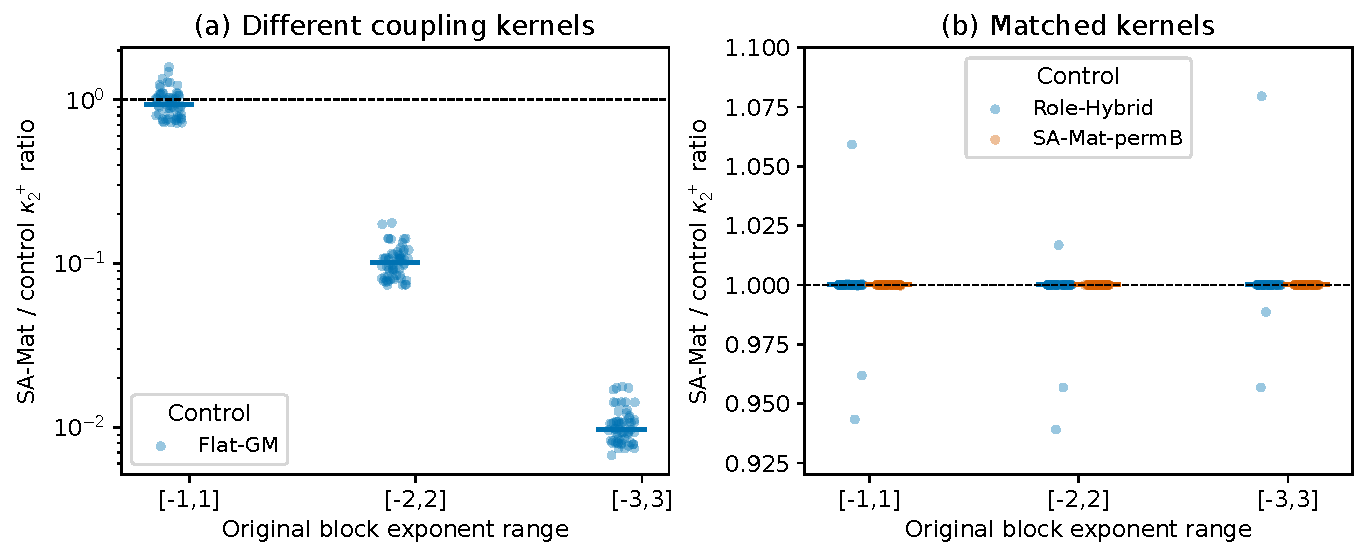
\includegraphics[width=\linewidth]{identifiability.pdf}
\caption{Fresh matrix audit. Each exponent range contains 60 generated instances. Panel (a)
changes the coupling kernel; panel (b) holds the kernels fixed and removes (Role-Hybrid) or
permutes (SA-Mat-permB) the block-scale information. Marks are individual ratios with
deterministic horizontal jitter; short horizontal segments are medians. The panels use different
vertical scales. Unscaled matrices, whose estimates approach binary64 resolution, enter no ratio;
all paired scaled diagnostics are below $6.5\times10^6$}
\label{fig:identifiability}
\end{figure}


\subsection{Completed-run gains are not failure-robust}
\label{subsec:results-operational}
On the 14 SG-Ter-Mer instances that every policy completed, Flat-GM used less solver work than
Base, with paired geometric-mean ratios 0.698 at 1\% gap and 0.682 at 0.1\% (bootstrap
intervals $[0.486,0.944]$ and $[0.470,0.925]$): about 30--32\% less work on that pool. The
fifteenth instance, instance077, completes under Base and times out under every scaled policy
at both gaps. Under PAR10 this single failure dominates: Base averages 116 and 134 seconds,
while every scaled policy averages between 1,216 and 1,218 seconds (Online Resource 1,
Table~S5). Scaling therefore produced a sizeable completed-run efficiency gain in this class,
but the gain was not robust to failure-sensitive aggregation. On the six instances of the class
that are free of the scenario defect the conditional gain is larger and, since instance077 is
not among them, the reversal disappears (Online Resource 1, Table~S4). The Simple class has no uniform ordering: Flat-GM
lowers mean PAR10 from 11.9 to 2.1 seconds at 1\% gap and raises it from 52.0 to 73.0 seconds
at 0.1\%. Role-Hybrid stays within one second of Flat-GM in all four cells.

\paragraph{Replication under a second seed and a second solver.} The reconstruction is one
solver at one seed. The same 30 instances, four policies, two gaps and 1,800-second limit were
rerun changing one factor at a time (Online Resource 1, Table~S6). Under Gurobi with seed 7 the
SG-Ter-Mer effort ratio of Flat-GM is 0.778 at a 1\% gap and 0.777 at 0.1\%, against 0.698 and
0.682 at seed 42: the conditional gain survives the change of seed. Under CPLEX at the original
seed, in its own deterministic effort metric, the same ratio is 1.078 and 1.077: it does not survive
the change of solver. On the Simple class the three conditions agree in direction, Flat-GM below
one at the loose gap and between 0.84 and 1.06 at the tight one, Flat-L2 above one in all six
cells. The instance that reverses the ordering, instance077, behaves differently in each
condition: under Gurobi at seed 7 every policy times
out, Base included, while under CPLEX the run that reaches the limit is Base at the 1\% gap and
Role-Hybrid at 0.1\%.
The completed-run gain of this class is therefore a property of a representation together with a
pipeline, and the failure that reversed the PAR10 ordering is not a stable property of the
instance either. Neither observation is surprising in the light of what is known about
performance variability in mixed-integer programming: Lodi and Tramontani
\cite{lodi2013variability} document changes of this order from perturbations that leave the
model mathematically unchanged, such as a different seed or a permuted formulation. A row
scaling is exactly such a perturbation. The seed-to-seed movement reported here, from 0.698 to
0.778, is of the same order as the effect being measured, which is why these numbers are
reported as a measured conditional gain on a fixed pool rather than as an estimate of
acceleration.

The two endpoints answer different questions: completed-run effort describes how a
representation affects the runs that finish, and PAR10 whether it changes which runs finish.
For the reconstructed campaign itself, with one seed and 15 fixed instances per class, the
result is a measured conditional gain, not a population estimate of acceleration; the two
sensitivity reruns reinforce that caution rather than providing population-level replication. The same runs also show why a stated budget is
needed to read residuals: an absolute residual of 4.97 on a zero-RHS equality of caso46e has an
activity-normalized value of $1.15\times10^{-7}$, and without an application budget neither
number establishes acceptance; \cref{tab:application-budget} supplies one.

\subsection{Budgets improve verification; acceptance is pipeline-dependent}
\label{subsec:results-budget}
\begin{figure}[!tb]
\centering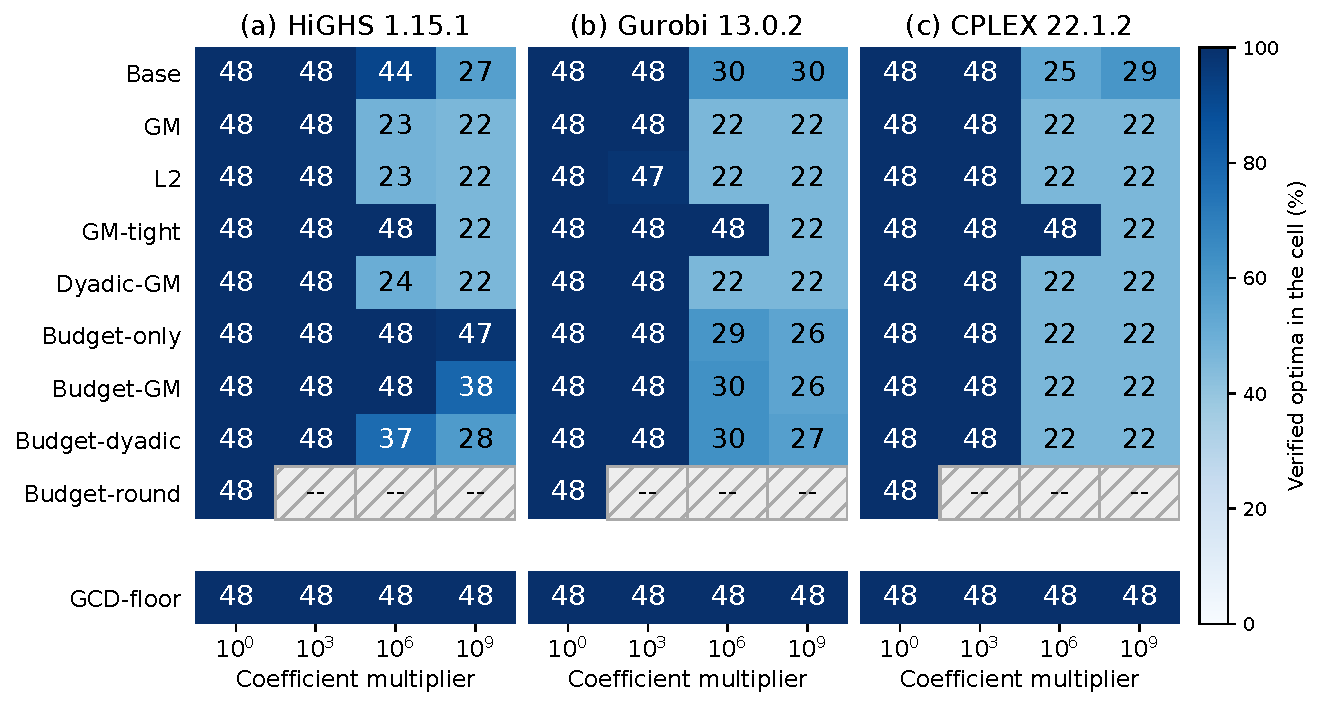
\includegraphics[width=.9\linewidth]{budget-verification.pdf}
\caption{Verified optima by coefficient multiplier. Each cell counts the configurations whose
returned point is a verified optimum, out of the 48 in that cell (three families, eight seeds,
two presolve settings); the shading is that count as a percentage, on the common scale at the
right. The fixed margin in \eqref{eq:stress-family} brings the continuous
feasibility boundary increasingly close to an integer activity. Hatched cells marked
\mbox{--} are abstentions, where the policy declines to export. The detached bottom row is
GCD-floor, the later integer-aware reformulation control, not a scaling policy.}
\label{fig:budget-verification}
\end{figure}
\begin{table}[!tb]
\centering\small
\caption{Paired verification outcomes on identical model, presolve and solver settings (192
per comparison and solver). ``$A$ only'' counts configurations verified under $A$ and not under
$B$.}\label{tab:budget-paired}
\resizebox{\textwidth}{!}{\begin{tabular}{lrrrrrr}
\toprule
& \multicolumn{2}{c}{HiGHS} & \multicolumn{2}{c}{Gurobi} & \multicolumn{2}{c}{CPLEX} \\
Comparison $A$ vs $B$ & $A$ only & $B$ only & $A$ only & $B$ only & $A$ only & $B$ only \\
\midrule
Budget-GM vs GM & 41 & 0 & 12 & 0 & 0 & 0 \\
Budget-dyadic vs Dyadic-GM & 19 & 0 & 13 & 0 & 0 & 0 \\
Budget-only vs GM & 50 & 0 & 11 & 0 & 0 & 0 \\
GM vs Base & 0 & 26 & 0 & 16 & 0 & 10 \\
Budget-only vs Base & 24 & 0 & 1 & 6 & 0 & 10 \\
Budget-GM vs Base & 15 & 0 & 1 & 5 & 0 & 10 \\
Budget-dyadic vs Base & 2 & 8 & 1 & 4 & 0 & 10 \\
GM-tight vs GM & 25 & 0 & 26 & 0 & 26 & 0 \\
Budget-only vs GM-tight & 25 & 0 & 4 & 19 & 0 & 26 \\
Budget-only vs Budget-GM & 9 & 0 & 0 & 1 & 0 & 0 \\
\bottomrule
\end{tabular}
}
\end{table}

These models are small, adversarial and built so that an integer point sits a fixed distance
from the continuous boundary, so the counts below compare policies on a deliberately hard
family; they are not estimates of how often a solver fails in practice.

The residual budget has a consistent effect within each scaling rule
(\cref{tab:budget-paired}). Plain GM centering loses verified optima relative to Base on all
three solvers, 26 configurations on HiGHS, 16 on Gurobi and 10 on CPLEX, with no gains. At
multipliers $10^6$ and $10^9$ it shrinks the fixed 0.1 margin of \eqref{eq:stress-family} below
the solver tolerance, and most of its failures (49 of 51 on HiGHS, 36 of 52 on Gurobi, 34 of 52
on CPLEX) return points that satisfy the exported tolerance while violating the original row by
more than the budget. Adding the budget to the same rule never lost a verified configuration on
any solver. It recovered 41 of them on HiGHS and 12 on Gurobi, and none on CPLEX, where a rule
and its budgeted version verify exactly the same configurations; the dyadic pair shows the same
pattern, 19, 13 and 0. The two comparisons say different things about the same factors. Plain
centering improves the numbers in the exported file and loses verified optima; the same rule
with a budget attached loses none. A representation can be numerically better without being
operationally safer, unless what safer means is stated in the units of the original model.

Relative to the unscaled model, the outcome depends on the pipeline: presolve, internal
scaling, tolerances and finite precision all intervene between the exported row and the
accepted point. The complete
counts for every policy and solver are in Online Resource 1, Table~S7. On HiGHS, Budget-only
verifies 191 of 192 configurations and Budget-GM 182, against 167 for Base and 141 for GM;
Budget-only gains 24 configurations over Base and loses none. On Gurobi, Budget-only verifies
151, Budget-GM 152 and Base 156. On CPLEX every scaled policy verifies 140 and Base 150: the
budget changes nothing there, and the ten configurations lost to scaling are lost with it and
without it. On both commercial solvers, tightening the two tolerances to $10^{-9}$ (GM-tight,
166 configurations on each of the three solvers) is the more effective intervention. The same
stored models and row factors thus lead to different acceptance in three pipelines, and the
budget helps where this experiment shows the greater sensitivity to the exported coefficients.

The gap between Budget-only and Budget-GM on HiGHS is informative in its own right. At
multipliers $10^6$ and $10^9$, the only ones at which their outcomes differ, the budget endpoint
is binding and Budget-GM selects that endpoint rounded inward, one unit in the last place (ulp)
away from Budget-only's factor. All ten discordant configurations, nine on HiGHS and one on Gurobi,
with none on CPLEX, have exactly this one-ulp difference. The nine-configuration gap therefore measures how
sensitive solver acceptance is to the last bit of a factor near a tolerance boundary, not an
effect of coefficient centering. The same sensitivity appears at a larger scale: Budget-dyadic,
which uses the nearest admissible power of two and exports every product exactly, verifies 161
configurations on HiGHS, 153 on Gurobi and 140 on CPLEX. Exact representation of the scaled row does not by
itself secure acceptance.

Two controls delimit the result. GCD division with RHS flooring verifies all 192 configurations
on each solver: it removes the deliberately narrow integer margin, whereas a budget controls
the original-unit meaning of an exported residual, so the budget result is a comparison among
scalings and not an advantage over integer-aware presolve. Budget-round, which reserves the
worst-case rounding term of \eqref{eq:rounding-budget}, verifies all 48 configurations it
accepts per solver and abstains on the other 144, including many that other policies solve
correctly. Its abstentions certify that the requested uniform contract cannot be asserted; they
are not solved instances, and \cref{fig:budget-verification} counts them separately.

\paragraph{The same contract on the application.} The 0.01 of the stress family is a test
parameter, but the dispatch rows carry interpretable units, so a budget can be stated in them.
For illustration, suppose the modeller declares 0.1\,MW for the rows that account for
generation and cap it by demand, 0.1\,MW for the piecewise-linear production envelopes, and 1{,}000\,m\textsuperscript{3}
--- a thousandth of a cubic hectometre --- for the reservoir water balances.
\Cref{tab:application-budget} applies \cref{prop:budget} to the 4,320 rows of caso46e that carry
those meanings, with $\epsilon=10^{-6}$ and the coefficient window $[10^{-9},10^{9}]$. The
admissible interval is wide, the geometric-mean factor lies inside it on every row, and the
residual the tolerance allows in original units stays five to nine orders of magnitude below the
declared budget. On this model the contract leaves the geometric-mean factor unchanged on
every row: it restricts which factors are admissible, as it must, but the geometric-mean choice
considered here already lies well inside that restriction. The budgets are declared rather than
measured, so the margin is also the sensitivity: scaling all six by a common multiplier, all
three kernels stay admissible on all 4,320 rows down to $10^{-4}$ and the two the comparison
turns on down to $10^{-5}$, which places the result far from the chosen numbers (Online Resource 1,
Table~S8).

Its content is in the reading of a residual. One family is written pre-scaled: the Baygorria
generation definition carries a coefficient of $10^7$ on the generation variable, so the same
0.1\,MW becomes a budget of $10^{6}$ in the units of that row. It is the family on which the
accepted Flat-L2 run of \cref{subsec:results-operational} leaves its largest residual, 4.97,
which against the row's own budget is a generation error of $5\times10^{-7}$\,MW. The residual
as written and the quantity it stands for differ by the seven orders of magnitude of that
coefficient, and only a budget carried with the row distinguishes them.

\begin{table}[tb]
\centering\small
\caption{A declared residual contract on the dispatch model, applied to the 4,320 rows of
caso46e whose units are interpretable. Budgets are stated by the modeller, not measured or
supplied by the operator. Admissible factors are the interval of \cref{prop:budget} for
$\epsilon=10^{-6}$ and coefficient limits $[10^{-9},10^{9}]$. The geometric-mean factor is
constant within every group except the tangents, where it ranges over $[1.99,2.33]$; the
column ``GM (med.)'' gives its median, and ``Worst resid.'' gives $\epsilon$ divided by the
\emph{smallest} factor of the group, the largest original-unit residual the tolerance allows
there, in the units of that group's budget. The two therefore coincide except on the tangents, where the worst residual
$5.0\times10^{-7}$ belongs to the row with factor 1.99 rather than to the median row, whose
residual is $4.7\times10^{-7}$. The last group is written pre-scaled, with a coefficient of $10^7$ on the generation
variable, so 0.1\,MW there is $10^{6}$ in the units of the row as written. The admissibility
check covers the three kernels the four policies use --- the unit factor, the geometric-mean
factor shown here and $1/\|a_r\|_2$ --- and every one of them is admissible on every row. The
archived admissibility check records the corresponding counts for each kernel.}
\label{tab:application-budget}
\resizebox{\textwidth}{!}{\begin{tabular}{lrrrr}
\toprule
Constraint group & Budget $\delta$ & Admissible factors & GM (med.) & Worst resid. \\
\midrule
Generation identities, demand cap & 0.1~MW & [$10^{-5}$, $10^{9}$] & 1 & $10^{-6}$ \\
Generation definition, Bonete/Palmar & 0.1~MW & [$10^{-5}$, $10^{9}$] & 1 & $10^{-6}$ \\
Production envelope tangents & 0.1~MW & [$10^{-5}$, $10^{9}$] & 2.14 & $5.0\times10^{-7}$ \\
Water balance, Bonete/Palmar & $10^{3}$~m\textsuperscript{3} & [$10^{-9}$, $2.8\times10^{5}$] & 0.0167 & $6.0\times10^{-5}$ \\
Water balance, Baygorria & $10^{3}$~m\textsuperscript{3} & [$10^{-9}$, $2.8\times10^{5}$] & $2.8\times10^{-4}$ & $3.6\times10^{-3}$ \\
Generation definition, Baygorria & $10^{6}$~row units & [$7.0\times10^{-8}$, 100] & $2.6\times10^{-3}$ & $3.8\times10^{-4}$ \\
\bottomrule
\end{tabular}
}
\end{table}

\section{Discussion}
\label{sec:discussion}
\subsection{What we learned}
\paragraph{Row scaling changes the exported representation, and part of that reaches the
solver.} With the basis held fixed, the representation alone moves the condition number of the
exported file by six to eight orders of magnitude in the median, and the kernel decides whether
it does. That figure describes the file. A solver-style equilibration applied to the same bases
recovers most of it --- ten to fourteen orders on the unscaled model --- and what the choice of
export is still worth afterwards is a factor of about six in two classes and two in the third.
The pre-export choice is not erased, because an infinity-norm equilibration does not undo a row
scaling, but it is worth far less than the file-level number suggests, and on one class it
inverts: the kernel that ranks last on the file ranks first after that equilibration.

\paragraph{The mechanism is simpler than the metadata explanation.} Under exact GM local
normalization, the extrema-based post-local block statistic carries no block-scale information
(\cref{prop:audit-collapse}), so the block-relative rule becomes Euclidean normalization of the
coupling rows. Separately, on a locally whitened triangular structure the optimal common factor
is $(1+\rho^2)^{-1/2}$ (\cref{prop:audit-triangular-optimum}); the two coincide when the
structure has a single coupling row.

\paragraph{Matching kernels is essential for attribution.} The original comparison changed the
coupling kernel together with the information used, and the fixed-basis audit shows how much a
kernel alone can change: identical coverage, representations orders of magnitude apart. A claim
that generator information improves preprocessing needs a kernel-matched control.

\paragraph{A condition number of an exported file does not rank scaling policies.} It is the
natural thing to measure, because it needs no optimizer and no license, and this paper measures
it on 306 models. What \cref{subsec:results-bridge} shows is that it should not be used to
choose between kernels: after a solver-style equilibration the ordering it gives is wrong in
sign on one of the three classes and compressed by six orders of magnitude on the others.
Anyone comparing pre-export scalings by a matrix diagnostic should report what remains of the
difference once that diagnostic is recomputed through such a step, which costs no optimizer
time. Whether a particular solver's own stage leaves more or less than the model used here is a
question this paper does not settle.

\paragraph{Residual budgets are a meaningful invariant quantity.} A residual budget carried
consistently with its row defines a contract that is invariant under consistent re-emission ---
the number changes with the row, the meaning does not --- and determines the admissible factors
exactly. In the
stress test, measured against the corresponding unbudgeted rule, it repaired the verification
losses of coefficient centering on two of the three solvers and cost nothing on the third;
measured against the unscaled model the outcome still depends on the pipeline. On the dispatch
model the same contract is easy to satisfy --- all three kernels the four policies use are
admissible on each of its 4,320 interpretable rows, with orders of magnitude to spare --- and
its work is in the reading of a residual, which without a stated unit says nothing. GCD division with RHS flooring verified every stress configuration, but it
answers a different question: it is an integer-aware reformulation that exploits the activity
lattice of integer rows, whereas a residual budget is a contract in original units that also
applies to continuous rows and to constraints admitting no such reduction.

\paragraph{Solver acceptance and effort are properties of the pipeline.} The same
representation reduced completed-run work and caused a timeout, the same factors were accepted
differently by the three pipelines, and a one-ulp change in a factor changed outcomes in one of
them. Pipeline, not solver: presolve, internal scaling, tolerances and finite precision all sit
between the exported row and the point that comes back, and the experiments here cannot
separate their contributions.

\subsection{Scope and limitations}
The operational evidence comes from one application: two instance classes and 15 fixed
instances per class, from the reconstructed campaign of \cref{subsec:design-operational}. The two
sensitivity reruns, under a second seed and a second solver, are enough to show that at least
one finding is configuration-dependent rather than a stable property of the representation, and
far too small to describe the population of configurations. The stress instances are small and
deliberately adversarial; their budget of 0.01 is a numerical test parameter, and the dispatch
budgets of \cref{tab:application-budget} are stated by us to show what the contract implies,
not supplied or validated by the operator. Solver outcomes depend on
the solver, its version and its settings. The collapse result concerns the extrema-based block
statistic after GM normalization; other block statistics, other kernels and physical scale
information are outside it, and on the operational models the coupling rows receive the same
factors under every GM-local policy, so ownership is tested only on synthetic matrices. Finally, row scaling cannot repair within-row
heterogeneity beyond the limit in \eqref{eq:budget-feasibility} or the integer-rounding
amplification in \eqref{eq:rounding-budget}.

\section{Conclusion}
External row scaling changes the exported representation a great deal and the representation
after a solver-style equilibration rather less. Holding one basis fixed, it moves the condition
number of the file by six to eight orders of magnitude in the median while preserving the MILP
in exact arithmetic, and the kernel determines whether this happens; after such an
equilibration, what the choice is still worth is a factor of a few. The difference is not
erased --- a row scaling is not in the kernel of an infinity-norm equilibration --- but the
file-level figure is not a measure of what necessarily survives solver-side scaling, and it
does not even order the kernels correctly.

Correct attribution changes the explanation of the gain. The advantage originally attributed to
block metadata is a coupling-kernel effect: exact GM local normalization erases the
extrema-based post-local block statistic, and the closed-form coupling factor of the idealized
triangular model, which reduces to Euclidean normalization in the single-row case, provides a
spectral explanation for it that uses no ownership information.

Residual budgets provide a constructive way to encode information that keeps its meaning in
original application units. They come with exact feasibility and incompatibility conditions, a
centered factor, invariance under re-emission, and explicit rounding and binary64 export
conditions, and in the stress experiment adding the residual budget to the same scaling rule
never reduced verification against that same unbudgeted rule, on any of the three solvers
tested.

What a solver does with a scaled representation still has to be measured, and its output still
has to be verified. The practical lesson is therefore not to avoid external scaling, but to make
it accountable, in three steps that cost no optimizer time: attribute its gains with
kernel-matched controls, measure them again through a solver-style equilibration before
believing the ordering they give, and state its accuracy contract in the model's own units so
that solver output can be verified against it.

\section*{Data and software availability}
The accompanying repository contains the C++ generator, frozen historical aggregates, the
reconstructed operational logs and analysis, the fixed-basis audit with its exports, bases and
independent verification, the exact-enumeration experiment, the row-factor implementation,
tests, and the scripts that generate the tables and vector figures. The current research
sources are distinguished from the historical draft, whose positive block-attribution claim is
superseded. All newly reported data are stored under
\texttt{results-revision/research-audit/}. No commercial solver is required to regenerate the
figures, rerun the fixed-basis audit, verify the saved binary solutions, or run the HiGHS stress
arm. Rerunning the Gurobi and CPLEX arms requires the corresponding licenses.

The repository is at \url{https://github.com/MathiasRodriguezCastro/structure-aware-row-scaling}.
The state reviewed here is the fixed release \texttt{v1.0-mpc-submission}, which carries three
archives: the manuscript sources, the source and data archive that is Online Resource~2, and the
bulk inputs of the fixed-basis audit, 5.18~GB of exported LP text and bases in a 337~MB
compressed file. Only the rebuild of all 1,530 bases from that text needs the last one; every
number reported here follows from the summaries in Online Resource~2.

\section*{Supplementary information}
Online Resource 1 provides the triangular-model proof, the fixed-basis audit protocol and
complete ranges, operational reconstruction details, frozen experiment protocols, arithmetic
implementation checks, and reproduction instructions. The accompanying source and data archive
is Online Resource 2.

\bibliographystyle{spmpsci}
\bibliography{research-references}

\section*{Acknowledgements}
The experiments reported in this paper were carried out using ClusterUY, the national
supercomputing facility of Uruguay (\url{https://cluster.uy}).

\section*{Statements and Declarations}
\paragraph{Funding.}
The author received no external funding, grant or material support for this work.
\paragraph{Competing interests.}
The author declares no financial or non-financial competing interests. No solver vendor
or software project discussed here had any role in the design, execution, analysis or
reporting of the study.
\paragraph{Author contributions.}
Mathias Rodr\'iguez Castro is the sole author and is responsible for the conception of
the study, the implementation, the experiments, the analysis and the manuscript. The
model generator used as the source of instances originates in his hydrothermal-dispatch
thesis work.
\paragraph{Ethics approval, consent and human or animal participants.}
Not applicable: the study involves no human participants, animals or personal data.
\paragraph{Use of AI assistance.}
AI assistants (OpenAI ChatGPT and Codex, and Anthropic Claude) were used as coding and
writing tools during the preparation of this work: for implementation and verification code, for
derivations and their review, for analysis of the literature, and for drafting and
editorial revision. Reported numerical results come from the stored computational runs,
and figures were generated programmatically from those data or the stated equations. The
author independently verified the mathematical arguments, the experimental design, the
computational results and the scientific conclusions, and takes full responsibility for
the manuscript.

\end{document}
